\title{\color{ladrillo}\bfseries De Abraham al Éxodo\\[4pt]\large\color{cafe}\mdseries Un pueblo creado desde la imposibilidad, llamado a bendecir y sostenido por una promesa de regreso}
\author{}\date{\color{sepia}Serie «Israel, el pueblo de Dios» · Estudio 1}
\begin{document}
\maketitle\thispagestyle{empty}

\begin{abstract}\noindent
Este primer estudio de la serie recorre la historia de Israel desde el llamado de Abram (Gn 12) hasta la salida de Egipto y el cántico del mar (Éx 15). Defiende dos tesis que acompañarán a toda la serie. La primera: Israel no nace de la fuerza de una etnia, sino de una palabra de Dios dirigida a una pareja estéril, y nace con una vocación hacia las naciones que el Sinaí formulará como «reino de sacerdotes y nación santa» (Éx 19:6). La segunda: la promesa de restauración no es un recurso tardío de los profetas, sino que está inscrita en el pacto con Abraham, que anuncia de antemano un destierro y un regreso (Gn 15:13–16). El estudio integra el texto hebreo, los datos arqueológicos sobre semitas en Egipto y sus límites, la memoria litúrgica judía (la Amidá, la Hagadá de Pésaj, el shofar de Rosh Hashaná) y la lectura que Isaías, Jeremías y Pablo hacen de Abraham y del Éxodo. Concluye que el Dios que «se acordó de su pacto con Abraham, con Isaac y con Jacob» (Éx 2:24) es el mismo que, según Pablo, mantiene a Israel «amado por causa de los padres» (Ro 11:28).
\par\smallskip\noindent\textbf{Palabras clave:} Abraham, pacto, Éxodo, remanente, restauración, Isaías, Jeremías, Romanos 11.
\end{abstract}

\section{Introducción}

¿Por qué Dios eligió un pueblo? La pregunta incomoda a lectores modernos, que sospechan favoritismo, y a muchos cristianos, que suponen que la elección de Israel fue un andamio retirado cuando se construyó la iglesia. Pablo la responde de otro modo: los israelitas siguen siendo aquellos «de quienes son la adopción, la gloria, los pactos, la promulgación de la ley, el culto y las promesas; de quienes son los padres» (Ro 9:4–5), y «los dones y el llamamiento de Dios son irrevocables» (Ro 11:29). Para entender esa afirmación hay que volver al principio, a Abraham.

La tesis de este estudio es doble. Primero, Israel es una creación de Dios, no una conquista humana: nace de Sara, que era estéril (Gn 11:30), y de una promesa que Abraham no vio cumplida en vida (Hch 7:5). Segundo, la historia de Israel trae inscrito desde su origen el ciclo de destierro y regreso: antes de que exista el pueblo, Dios anuncia que la descendencia de Abram será extranjera y oprimida, y que «en la cuarta generación volverán acá» (Gn 15:16). Lo que los profetas dirán después sobre Babilonia y sobre la dispersión es la ampliación de ese primer patrón.

\begin{center}\small
\renewcommand{\arraystretch}{1.3}
\begin{tabular}{>{\RaggedRight\arraybackslash}p{3.1cm}>{\RaggedRight\arraybackslash}p{5.6cm}>{\RaggedRight\arraybackslash}p{5.2cm}}
\toprule
\textbf{Eje de la serie} & \textbf{Pregunta en esta etapa} & \textbf{Textos centrales}\\
\midrule
Nación santa y reino de sacerdotes & ¿Para qué fue llamado Abraham y qué función tiene su descendencia ante las naciones? & Gn 12:1–3; 18:18–19; 22:18; Éx 4:22; 19:4–6\\
Promesa de restauración & ¿Dónde aparece por primera vez el patrón de exilio y regreso, y en qué se funda? & Gn 15:13–16; 46:3–4; 50:24–25; Éx 2:24; 6:6–8\\
Proyección profética y paulina & ¿Cómo releen Isaías, Jeremías y Pablo a Abraham y al Éxodo? & Is 41:8; 51:1–3; Jer 31:35–37; 33:25–26; Ro 4; 11:16, 28–29\\
\bottomrule
\end{tabular}\end{center}

\begin{nota}[Sobre traducción, numeración y fechas]
Las citas bíblicas son traducción propia desde el texto hebreo (BHS) y griego (NA28); la Septuaginta se cita según Rahlfs-Hanhart. Cuando la numeración hebrea difiere de la española, se da la española y la hebrea entre corchetes, por ejemplo Gn 32:28 [32:29]. Las fechas se indican como a.\,e.\,c. (antes de la era común) y e.\,c.
\end{nota}

\section{Marco cronológico}

La Biblia ofrece dos datos para fechar el período. Primero, 1~R 6:1 sitúa la salida de Egipto 480 años antes del cuarto año de Salomón; con el cuarto año de Salomón hacia el 966 a.\,e.\,c., el Éxodo caería hacia el 1446 a.\,e.\,c. («datación temprana»). Segundo, Éx 12:40 da 430 años de permanencia. Muchos historiadores prefieren una «datación tardía», en el siglo \textsc{xiii} a.\,e.\,c., porque Éx 1:11 menciona la ciudad de Ramsés, que suele identificarse con Pi-Ramsés (Qantir), construida bajo Ramsés~II (Hoffmeier, 1997; Kitchen, 2003). Quienes defienden la fecha temprana responden que el nombre pudo actualizarse en la transmisión, como ocurre con «Dan» en Gn 14:14. El debate sigue abierto y no se resolverá aquí; lo que importa para este estudio es la secuencia, no el año exacto.

\begin{nota}[Precisión textual: los 430 años de Éx 12:40]
El Texto Masorético dice que Israel habitó en Egipto 430 años. La Septuaginta y el Pentateuco samaritano leen «en la tierra de Egipto \emph{y en la tierra de Canaán}», de modo que los 430 años cubren también la etapa de los patriarcas. Pablo cuenta 430 años desde la promesa hasta la ley (Gá 3:17), lo que concuerda con la lectura larga. Flavio Josefo da 215 años en Egipto (\emph{Antigüedades} 2.15.2), y la cronología rabínica tradicional cuenta los 400 años de Gn 15:13 desde el nacimiento de Isaac y deja unos 210 años en Egipto (Seder Olam Rabbah; Rashi sobre Éx 12:40; Guggenheimer, 1998). Este estudio sigue el TM en la traducción y señala la lectura alternativa.
\end{nota}

\begin{center}
\begin{tikzpicture}[x=1cm,y=1cm]
\draw[line width=1.6pt,cafe,-{Latex[length=3mm]}] (0,0) -- (15.4,0);
\foreach \x/\t/\b in {0.6/{Llamado de Abram}/{Gn 12:1--3},
                      2.7/{Pacto entre las piezas}/{Gn 15},
                      4.8/{Isaac, hijo de la promesa}/{Gn 21:1--7},
                      6.9/{Jacob es llamado Israel}/{Gn 32:28 [32:29]},
                      9.0/{Descenso a Egipto}/{Gn 46:1--7},
                      11.1/{Opresión y clamor}/{Éx 1--2},
                      13.2/{Pascua y salida}/{Éx 12--15},
                      15.0/{Sinaí}/{Éx 19 (Est. 2)}}{
  \fill[oro] (\x,0) circle (4pt);
  \node[above,font=\scriptsize\bfseries,text=ladrillo,text width=1.9cm,align=center] at (\x,0.2) {\t};
  \node[below,font=\tiny,text=sepia,text width=1.8cm,align=center] at (\x,-0.2) {\b};}
\draw[decorate,decoration={brace,amplitude=5pt,mirror},sepia] (0.4,-0.85) -- (7.1,-0.85) node[midway,below=5pt,font=\scriptsize\itshape]{Patriarcas en Canaán: la promesa};
\draw[decorate,decoration={brace,amplitude=5pt,mirror},sepia] (8.8,-0.85) -- (13.4,-0.85) node[midway,below=5pt,font=\scriptsize\itshape]{Egipto: el primer exilio y su fin};
\end{tikzpicture}\\[2pt]
{\footnotesize\color{sepia}\textit{Nota.} Elaboración propia. Secuencia narrativa; las fechas absolutas están en debate (véase el texto).}
\end{center}

\section{Contexto histórico y arqueológico}

\subsection{De Ur a Harán y a Canaán}
Gn 11:31 hace salir a Taré y a Abram «de Ur de los caldeos» hacia Harán. Ur, en el sur de Mesopotamia, fue excavada por Leonard Woolley entre 1922 y 1934 y era una de las grandes ciudades de su tiempo. El calificativo «de los caldeos» refleja la denominación de una época posterior, cuando los caldeos dominaban la región; una tradición judía e islámica antigua prefiere identificar Ur con Urfa, en el norte, cerca de Harán (Sarna, 1989). Harán sí está bien atestiguada como centro de culto a la luna, igual que Ur, un dato que da contexto a Jos 24:2: «vuestros padres habitaron antiguamente al otro lado del río\ldots\ y servían a otros dioses». El llamado de Abram es, por tanto, una ruptura religiosa además de geográfica.

\begin{center}\begin{minipage}{\linewidth}\centering
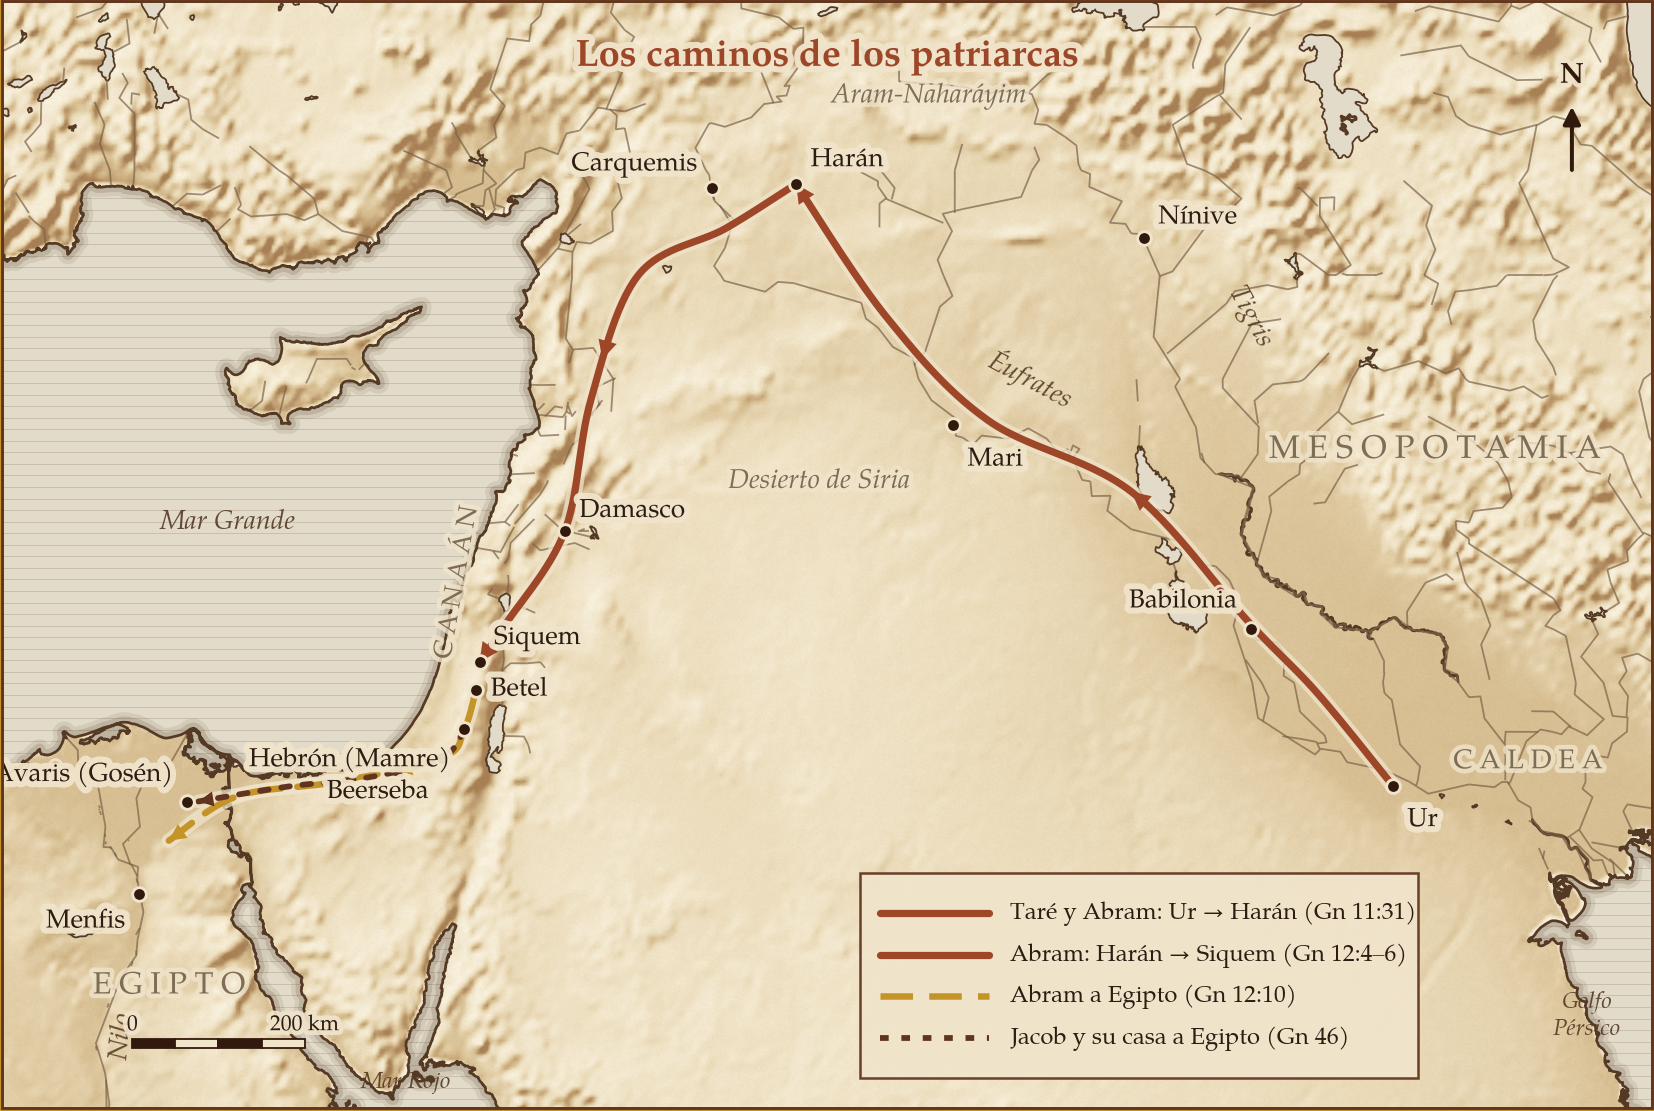
\includegraphics[width=1\linewidth]{mapa_patriarcas.png}\\[2pt]
{\footnotesize\color{sepia}\textit{Nota.} Elaboración propia: costas, lagos y ríos GSHHS/WDB y relieve sombreado (Basemap); ubicaciones antiguas aproximadas. }
\end{minipage}\end{center}


\subsection{Los patriarcas y el debate sobre su historicidad}
A mediados del siglo \textsc{xx} se citaban costumbres de los archivos de Nuzi y Mari (adopción, herederos sustitutos, nombres amorreos) como paralelos que situarían a los patriarcas en el Bronce Medio. Thompson (1974) y Van Seters (1975) mostraron que muchos de esos paralelos eran débiles o también tardíos, y una parte de la academia concluyó que los relatos no pueden fecharse. Otros autores sostienen que los nombres, los precios de esclavos y las formas de pacto encajan mejor en el segundo milenio que en el primero (Kitchen, 2003). Lo prudente es distinguir: la arqueología no ha encontrado a Abraham, y no cabe esperarlo de un pastor seminómada; pero el mundo que describe Génesis (migraciones de grupos semitas, pactos de tratado, descenso a Egipto en tiempos de hambre) es históricamente verosímil.

\begin{nota}[Precisión arqueológica: los camellos de Gn 12:16]
Gn 12:16 menciona camellos entre los bienes de Abram. Un estudio de restos óseos en el valle del Aravá sitúa la introducción del camello doméstico en el sur del Levante hacia el siglo \textsc{x} a.\,e.\,c. (Sapir-Hen y Ben-Yosef, 2013), y algunos lo leen como anacronismo. Otros recuerdan que la domesticación es anterior en Arabia y que un uso limitado por parte de grupos móviles no deja necesariamente huella en los asentamientos. Es un punto en debate, no una prueba en ningún sentido.
\end{nota}

\subsection{Semitas en Egipto}
Varios hallazgos muestran que la presencia de semitas del Levante en Egipto era corriente en el período en que se sitúa a José y a la familia de Jacob:
\begin{itemize}
\item \textbf{Pintura de Beni Hasan} (tumba de Jnumhotep~II, c. 1890 a.\,e.\,c.): un grupo de 37 «asiáticos» (\emph{aamu}) encabezados por un jefe llamado Abisha llega a Egipto con mercancías, vestidos de colores (Newberry, 1893). No es la familia de Jacob, pero muestra cómo eran estos grupos.
\item \textbf{Avaris} (Tell el-Dab\textquoteright a), en el delta oriental, zona de Gosén: las excavaciones de Manfred Bietak documentan desde c. 1800 a.\,e.\,c. una población de origen cananeo que creció hasta dar origen a la dinastía de los hicsos (Bietak, 1996).
\item \textbf{Papiro Brooklyn 35.1446}: una lista de siervos de una casa egipcia de fines del Reino Medio; cerca de la mitad tiene nombres semíticos del noroeste, entre ellos una mujer llamada \emph{Shifra}, el mismo nombre de una de las parteras de Éx 1:15 (Hayes, 1955; Albright, 1954). No se trata de la misma persona; el dato muestra que esos nombres eran comunes entre los semitas que servían en Egipto.
\item \textbf{Estela de Merneptah} (c. 1208 a.\,e.\,c.): el faraón dice que «Israel está devastado; su descendencia no existe». Es la mención extrabíblica más antigua de Israel, escrita con el determinativo de pueblo, no de territorio. Prueba que hacia fines del siglo \textsc{xiii} a.\,e.\,c. Israel ya era un pueblo identificable en Canaán.
\end{itemize}
Ninguna fuente egipcia narra el Éxodo, y esto se usa a menudo como argumento en contra. Hoffmeier (1997) responde que las inscripciones reales egipcias no registraban derrotas y que el delta, por su humedad, conserva muy mal los papiros; además, varios detalles del relato (nombres egipcios como Moisés, Putifar o Zafnat-panea, el trabajo con ladrillos y paja de Éx 5, la geografía del delta oriental) se ajustan a lo que se conoce de Egipto. La ausencia de evidencia directa obliga a la cautela, no autoriza a negar el relato.

\section{Desarrollo bíblico}

\subsection{El llamado de Abram: un nombre recibido, no fabricado}
El llamado de Gn 12 llega justo después de Babel, donde los hombres dicen: «Hagámonos un nombre» (\heb{וְנַעֲשֶׂה־לָּנוּ שֵׁם}, Gn 11:4). La respuesta de Dios a una humanidad dispersa no es otra torre, sino un hombre al que Él mismo promete engrandecer el nombre:

\hebverso{וְאֶעֶשְׂךָ לְגוֹי גָּדוֹל וַאֲבָרֶכְךָ וַאֲגַדְּלָה שְׁמֶךָ וֶהְיֵה בְּרָכָה\\
וַאֲבָרְכָה מְבָרְכֶיךָ וּמְקַלֶּלְךָ אָאֹר וְנִבְרְכוּ בְךָ כֹּל מִשְׁפְּחֹת הָאֲדָמָה}
\begin{cita}Haré de ti una nación grande, te bendeciré y engrandeceré tu nombre, y sé tú una bendición. Bendeciré a los que te bendigan, y al que te maldiga maldeciré; y en ti serán benditas todas las familias de la tierra.\fuente{(Gn 12:2--3)}\end{cita}

Tres rasgos del texto marcan toda la serie. Primero, la iniciativa es de Dios: los verbos están en primera persona («haré», «bendeciré», «engrandeceré»). Segundo, la «nación» (\heb{גּוֹי}, \emph{goy}) prometida no es un fin en sí misma: el imperativo «sé una bendición» (\heb{וֶהְיֵה בְּרָכָה}, \emph{ve-heyé berajá}) le da una tarea. Tercero, el horizonte es universal: «todas las familias de la tierra», las mismas que Gn 10 enumeró y Gn 11 dispersó. La elección de uno tiene como meta la bendición de todos.

\begin{nota}[Precisión filológica: \emph{nivrejú}]
La forma \heb{וְנִבְרְכוּ} (\emph{ve-nivrejú}, nifal) puede entenderse como pasiva («serán benditas») o como reflexiva («se bendecirán», es decir, usarán tu nombre al bendecir). En Gn 22:18 y 26:4 aparece el hitpael \heb{וְהִתְבָּרְכוּ}, que favorece el sentido reflexivo. La Septuaginta tradujo en pasiva (\grc{ἐνευλογηθήσονται}), y Pablo sigue esa lectura en Gá 3:8. Ambas lecturas mantienen la idea central: el destino de las naciones queda ligado a Abraham.
\end{nota}

\subsection{El pacto entre las piezas (Gn 15)}
Gn 15 es el capítulo decisivo para esta serie. Comienza con la fe de Abram:

\hebverso{וְהֶאֱמִן בַּיהוָה וַיַּחְשְׁבֶהָ לּוֹ צְדָקָה}
\begin{cita}Y creyó a YHWH, y él se lo contó por justicia.\fuente{(Gn 15:6)}\end{cita}

El verbo \heb{הֶאֱמִן} (\emph{he'emín}, de la raíz \emph{'mn}, la misma de \emph{amén} y \emph{emuná}) significa apoyarse en alguien como en algo firme. Pablo construirá sobre este versículo su argumento de Ro 4 y Gá 3.

Después viene el rito: Abram parte animales y Dios, en forma de «horno humeante y antorcha de fuego», pasa solo entre las mitades (Gn 15:17). En los tratados del antiguo Cercano Oriente, quien pasaba entre los animales partidos se maldecía a sí mismo si rompía el pacto; Jer 34:18–20 conserva ese sentido. Que solo Dios pase indica que Él asume la obligación. La tradición judía llama a este pasaje \emph{berit bein ha-betarim}, «el pacto entre las piezas».

En medio del rito aparece el primer anuncio de exilio y regreso de la Biblia:

\hebverso{יָדֹעַ תֵּדַע כִּי־גֵר יִהְיֶה זַרְעֲךָ בְּאֶרֶץ לֹא לָהֶם וַעֲבָדוּם וְעִנּוּ אֹתָם אַרְבַּע מֵאוֹת שָׁנָה}
\begin{cita}Ten por cierto que tu descendencia será extranjera en una tierra que no es suya; los harán servir y los oprimirán cuatrocientos años. Pero también a la nación a la que servirán la juzgaré yo, y después de esto saldrán con gran riqueza [\ldots]. Y en la cuarta generación volverán acá.\fuente{(Gn 15:13--14, 16)}\end{cita}

El verbo de Gn 15:16 es \heb{יָשׁוּבוּ} (\emph{yashuvu}), de la raíz \heb{שׁוּב} (\emph{shuv}), «volver». Es el verbo del regreso del exilio y también el del arrepentimiento (\emph{teshuvá}). Desde aquí, la esperanza de Israel se dirá con él: Dt 30:3 («YHWH tu Dios hará volver tu cautividad»), Jer 29:14, Jer 31:16–17. El patrón queda fijado antes de que exista el pueblo: \destacar{promesa, destierro, juicio sobre el opresor, regreso}.

\subsection{Pacto perpetuo, nombre nuevo y circuncisión (Gn 17)}
En Gn 17 el pacto se llama \emph{perpetuo}:

\hebverso{וַהֲקִמֹתִי אֶת־בְּרִיתִי בֵּינִי וּבֵינֶךָ וּבֵין זַרְעֲךָ אַחֲרֶיךָ לְדֹרֹתָם לִבְרִית עוֹלָם}
\begin{cita}Estableceré mi pacto entre mí y ti, y tu descendencia después de ti, por sus generaciones, como pacto perpetuo.\fuente{(Gn 17:7)}\end{cita}

El nombre cambia de Abram a Abraham, explicado como «padre de una multitud de naciones» (\heb{אַב־הֲמוֹן גּוֹיִם}, \emph{av hamón goyim}, Gn 17:5). Pablo cita este versículo en Ro 4:17 para sostener que Abraham es padre de los creyentes de las naciones. La señal del pacto, la circuncisión, marca la carne de la descendencia; los profetas y Moisés añadirán que Dios quiere circuncidar el corazón (Dt 10:16; 30:6; Jer 4:4).

\subsection{La Akedá: la promesa entregada y devuelta (Gn 22)}
Isaac es el hijo de la imposibilidad: Sara era estéril y ambos eran ancianos (Gn 18:11–14). En Gn 22 Dios pide a Abraham que ofrezca precisamente al hijo en quien descansa la promesa. Abraham obedece y Dios provee el carnero; el lugar recibe el nombre \heb{יְהוָה יִרְאֶה} (\emph{YHWH yiré}, «YHWH proveerá/verá», Gn 22:14). Dios renueva entonces la promesa con juramento: «en tu descendencia serán benditas todas las naciones de la tierra» (Gn 22:18). La tradición identifica el «monte Moriah» con el monte del templo, apoyada en 2 Cr 3:1; la carta a los Hebreos lee la escena como figura de resurrección (Heb 11:17–19).

\subsection{Jacob llamado Israel}
La promesa pasa a Isaac y luego a Jacob, no por mérito sino por elección: Pablo lo subraya con Ro 9:10–13. En Peniel, Jacob lucha y recibe un nombre nuevo:

\begin{cita}No se dirá más tu nombre Jacob, sino Israel, porque has luchado con Dios y con los hombres, y has prevalecido.\fuente{(Gn 32:28 [32:29])}\end{cita}

El texto explica el nombre con el verbo \emph{sará}, «luchar»: \emph{Yisra-El}. Como en muchas etimologías bíblicas, se trata de una explicación por sonido, no de un análisis lingüístico; el sentido gramatical más probable es «Dios lucha» o «que Dios prevalezca» (Sarna, 1989). El pueblo entero llevará el nombre de un hombre herido que no soltó a Dios hasta ser bendecido. En Gn 35:11 Dios le promete «una nación y un conjunto de naciones» (\heb{גּוֹי וּקְהַל גּוֹיִם}, \emph{goy u-qehal goyim}), y en Gn 48:19 Jacob dice que la descendencia de Efraín será «plenitud de las naciones» (\heb{מְלֹא־הַגּוֹיִם}, \emph{melo ha-goyim}). Esta última expresión será importante cuando la serie trate la división del reino y Romanos 11; aquí basta con registrarla.

\subsection{José y el primer remanente}
La historia de José explica cómo la familia llega a Egipto. Cuando se da a conocer a sus hermanos, José interpreta toda su historia como providencia:

\hebverso{לָשׂוּם לָכֶם שְׁאֵרִית בָּאָרֶץ וּלְהַחֲיוֹת לָכֶם לִפְלֵיטָה גְּדֹלָה}
\begin{cita}Dios me envió delante de vosotros para preservaros un remanente en la tierra y para daros vida por medio de una gran liberación.\fuente{(Gn 45:7)}\end{cita}

Aquí aparece por primera vez aplicada a la familia de Israel la palabra \heb{שְׁאֵרִית} (\emph{she'erit}, «remanente»), que Isaías convertirá en un concepto teológico central (Is 10:20–22) y que Pablo retomará: «ha quedado un remanente escogido por gracia» (Ro 11:5). La primera vez que Israel es «remanente», lo es para sobrevivir y para que otros vivan: José alimenta a Egipto y a «toda la tierra» (Gn 41:57).

\subsection{Del descenso al Éxodo}
Antes del descenso, Dios habla a Jacob en Beerseba:

\hebverso{אָנֹכִי אֵרֵד עִמְּךָ מִצְרַיְמָה וְאָנֹכִי אַעַלְךָ גַם־עָלֹה}
\begin{cita}Yo descenderé contigo a Egipto, y yo también te haré subir de nuevo.\fuente{(Gn 46:4)}\end{cita}

El exilio no separa a Israel de su Dios: Dios baja con él. Al morir, José hace jurar a sus hermanos que llevarán sus huesos a la tierra, porque «Dios ciertamente os visitará» (\heb{פָּקֹד יִפְקֹד}, \emph{paqod yifqod}, Gn 50:24–25). Moisés cumplirá el juramento (Éx 13:19) y Hebreos lo cuenta como acto de fe (Heb 11:22).

Éxodo comienza con la multiplicación del pueblo (Éx 1:7, eco de Gn 1:28), la opresión con ladrillo y barro (Éx 1:14) y el clamor. La respuesta de Dios se explica por el pacto:

\hebverso{וַיִּזְכֹּר אֱלֹהִים אֶת־בְּרִיתוֹ אֶת־אַבְרָהָם אֶת־יִצְחָק וְאֶת־יַעֲקֹב}
\begin{cita}Y oyó Dios su gemido, y se acordó Dios de su pacto con Abraham, con Isaac y con Jacob.\fuente{(Éx 2:24)}\end{cita}

«Acordarse» (\heb{זָכַר}, \emph{zajar}) no significa recuperar un dato olvidado, sino actuar a favor de alguien en virtud de un compromiso. En la zarza, Dios encarga a Moisés decir a los ancianos las mismas palabras de José: \heb{פָּקֹד פָּקַדְתִּי} (\emph{paqod paqadti}, «ciertamente os he visitado», Éx 3:16). Una tradición midrásica dice que esa fórmula era la señal de redención transmitida desde José, por la cual los ancianos reconocerían al verdadero libertador (Pirqé de-Rabí Eliézer, cap. 48; Friedlander, 1916).

Antes de la primera plaga, Dios llama a Israel «mi hijo, mi primogénito» (\heb{בְּנִי בְכֹרִי יִשְׂרָאֵל}, Éx 4:22). En Éx 6:6–8 promete la liberación con una cadena de verbos: «os sacaré», «os libraré», «os redimiré», «os tomaré por pueblo», «os introduciré en la tierra». La Pascua (Éx 12) y el paso del mar (Éx 14–15) cumplen los cuatro primeros. Con Israel sale también «una multitud mixta» (\heb{עֵרֶב רַב}, \emph{érev rav}, Éx 12:38): desde la primera redención, gente de otras naciones se une al pueblo, y la ley de la Pascua prevé su incorporación (Éx 12:48–49).

\section{Israel como nación santa y reino de sacerdotes}

La fórmula de Éx 19:6, «vosotros me seréis un reino de sacerdotes y una nación santa» (\heb{מַמְלֶכֶת כֹּהֲנִים וְגוֹי קָדוֹשׁ}, \emph{mamléjet kohaním ve-goy qadosh}), se pronuncia en el Sinaí y será el centro del Estudio~2. Pero su contenido ya está presente en la historia patriarcal. Un sacerdote es un mediador: lleva a Dios ante el pueblo y al pueblo ante Dios. Eso hacen los patriarcas:

\begin{itemize}
\item \textbf{Abraham edifica altares e invoca el nombre} de YHWH en cada etapa del camino (Gn 12:7–8; 13:18).
\item \textbf{Intercede por otros pueblos}: por Sodoma (Gn 18:22–33) y por Abimelec, rey filisteo, de quien Dios dice: «es profeta, y orará por ti» (Gn 20:7).
\item \textbf{Es elegido para enseñar}: «para que mande a sus hijos y a su casa después de sí que guarden el camino de YHWH, haciendo justicia y juicio» (Gn 18:19). La bendición de las naciones pasa por un pueblo que practica la justicia.
\item \textbf{José preserva la vida de las naciones} en la hambruna (Gn 41:57; 50:20).
\item \textbf{Israel es el primogénito} (Éx 4:22). En la familia antigua, el primogénito representaba a los hermanos y heredaba una función de liderazgo; en Israel los primogénitos fueron consagrados a Dios y luego sustituidos por los levitas (Éx 13:2; Nm 3:12). Llamar a Israel «primogénito» implica que hay otros hijos, las naciones, a quienes este hijo debe representar.
\end{itemize}

El material de estudio de la congregación resume el llamamiento de Israel en cinco puntos: reino de sacerdotes y nación santa (Éx 19:6), luz para las naciones (Is 49:6), custodio de la palabra de Dios (Dt 4:5–8; Sal 147:19–20; Ro 3:1–2), testigo de la fidelidad de Dios (Is 43:10–12) y heredero de la tierra (Gn 13:14–15) (Departamento de Educación, s.\,f.). Esta etapa contiene en germen los cinco.

Isaías retomará la vocación sacerdotal como meta de la restauración: «vosotros seréis llamados sacerdotes de YHWH; ministros de nuestro Dios os dirán» (\heb{וְאַתֶּם כֹּהֲנֵי יְהוָה תִּקָּרֵאוּ}, Is 61:6). Y la extenderá a las naciones: de entre ellas tomará Dios «sacerdotes y levitas» (Is 66:21). Pedro aplicará Éx 19:6 en su forma griega (\grc{βασίλειον ἱεράτευμα, ἔθνος ἅγιον}) a los creyentes de la diáspora (1~P 2:9). Para leer bien ese texto hay que recordar su origen: no anula a Israel, sino que muestra a qué se incorporan los creyentes.

\section{Aporte de la tradición judía}

La memoria judía de esta etapa se conserva menos en tratados que en la liturgia y el midrash. Conviene distinguir lo que dice el texto bíblico de lo que la tradición desarrolla.

\subsection{Abraham en el midrash}
\begin{itemize}
\item \textbf{El rompedor de ídolos.} Bereshit Rabbah 38:13 cuenta que Abram, hijo de un fabricante de ídolos, rompió las imágenes del taller de su padre. Es una narración haggádica, no un dato histórico, pero expresa lo que Jos 24:2 deja implícito: el llamado de Abram es una salida de la idolatría.
\item \textbf{«Abram el hebreo».} Gn 14:13 llama a Abram \heb{הָעִבְרִי} (\emph{ha-ivrí}). Bereshit Rabbah 42:8 relaciona el término con \emph{éver}, «el otro lado»: el mundo entero estaba de un lado y Abram del otro. Es un juego de palabras, pero describe bien la vocación de un pueblo apartado.
\item \textbf{Las diez pruebas.} La Mishná enseña que «con diez pruebas fue probado Abraham, nuestro padre, y las superó todas» (Avot 5:3).
\end{itemize}

\subsection{Los padres en la oración diaria}
La primera bendición de la Amidá, la oración central del judaísmo que se recita tres veces al día, se llama \emph{Avot}, «los padres»:

\hebverso{אֱלֹהֵי אַבְרָהָם אֱלֹהֵי יִצְחָק וֵאלֹהֵי יַעֲקֹב \foreignlanguage{spanish}{[\ldots]} וְזוֹכֵר חַסְדֵי אָבוֹת וּמֵבִיא גּוֹאֵל לִבְנֵי בְנֵיהֶם}
\begin{cita}Dios de Abraham, Dios de Isaac y Dios de Jacob [\ldots] que se acuerda de las bondades de los padres y trae un redentor a los hijos de sus hijos.\fuente{(Amidá, primera bendición; Sacks, 2009)}\end{cita}

La oración une exactamente los dos ejes de esta serie: la memoria del pacto con los padres y la esperanza de un redentor. Es el concepto rabínico de \emph{zejut avot}, «el mérito de los padres». Pablo dice algo cercano, aunque con otro fundamento, cuando afirma que Israel es «amado por causa de los padres» (Ro 11:28): para Pablo, la razón no es el mérito de los patriarcas, sino la fidelidad de Dios a lo que les prometió.

\subsection{La Akedá y el shofar}
En Rosh Hashaná se leen Gn 21 y 22, y se toca el shofar, preferentemente un cuerno de carnero. El Talmud lo explica así: «Tocad delante de mí con un cuerno de carnero, para que me acuerde de vosotros de la atadura de Isaac hijo de Abraham» (Rosh Hashaná 16a). La Akedá queda asociada al juicio de Dios y a su memoria compasiva.

\subsection{Pésaj: memoria que se vuelve esperanza}
La Mishná establece: «en cada generación, cada persona está obligada a verse a sí misma como si hubiera salido de Egipto» (Pesajim 10:5). La Hagadá abre el relato con Dt 26:5, «un arameo a punto de perecer fue mi padre», y recorre la historia desde Abraham. Las cuatro copas del Séder se relacionan desde antiguo con los cuatro verbos de redención de Éx 6:6–7 (Talmud de Jerusalén, Pesajim 10:1). La quinta expresión, «os introduciré en la tierra» (Éx 6:8), quedó ligada en la costumbre posterior a la copa de Elías, el profeta que anuncia la redención futura. El Séder termina con «el año próximo en Jerusalén». La liturgia convierte el primer Éxodo en promesa de un Éxodo final.

\subsection{La Shejiná en el exilio}
A partir de Gn 46:4 («yo descenderé contigo»), los rabinos enseñaron que la presencia de Dios acompaña a Israel en sus destierros: «a todo lugar adonde fueron desterrados, la Shejiná fue con ellos: fueron desterrados a Egipto, y la Shejiná con ellos; a Babilonia, y la Shejiná con ellos» (Meguilá 29a). La enseñanza recorre las etapas que esta serie estudiará.

\section{La promesa de restauración}

\subsection{Textos fundantes en la Torá}
Los textos de esta etapa forman un patrón que los profetas retomarán:

\begin{center}\small
\renewcommand{\arraystretch}{1.3}
\begin{tabular}{>{\RaggedRight\arraybackslash}p{2.6cm}>{\RaggedRight\arraybackslash}p{5.2cm}>{\RaggedRight\arraybackslash}p{6.1cm}}
\toprule
\textbf{Texto} & \textbf{Promesa} & \textbf{Proyección}\\
\midrule
Gn 15:13--16 & Destierro, juicio del opresor, regreso (\emph{shuv}) & Dt 30:1--5; Jer 29:10--14\\
Gn 17:7 & Pacto perpetuo con la descendencia & Jer 31:35--37 [31:34--36]; Ro 11:29\\
Gn 45:7 & Un remanente preservado & Is 10:20--22; Ro 9:27; 11:5\\
Gn 46:4 & Dios baja al exilio y hace subir & Is 43:2; Ez 11:16\\
Gn 50:24 & «Dios ciertamente os visitará» & Éx 3:16; Lc 1:68\\
Éx 2:24 & Dios se acuerda del pacto con los padres & Lv 26:42--45; Lc 1:72--73\\
Éx 6:6--8 & Sacar, librar, redimir, tomar, introducir & Is 43:1; Jer 16:14--15\\
\bottomrule
\end{tabular}\end{center}

El texto más claro dentro de la propia Torá es Lv 26. Después de anunciar el destierro por la infidelidad, Dios dice:

\hebverso{וְזָכַרְתִּי אֶת־בְּרִיתִי יַעֲקוֹב וְאַף אֶת־בְּרִיתִי יִצְחָק וְאַף אֶת־בְּרִיתִי אַבְרָהָם אֶזְכֹּר וְהָאָרֶץ אֶזְכֹּר}
\begin{cita}Me acordaré de mi pacto con Jacob, y también de mi pacto con Isaac, y también de mi pacto con Abraham me acordaré, y de la tierra me acordaré.\fuente{(Lv 26:42)}\end{cita}

El orden invertido (Jacob, Isaac, Abraham) remonta la historia hasta el origen. La restauración se funda en el pacto con los padres, no en el mérito de la generación desterrada.

\subsection{Abraham y el Éxodo en Isaías}
Isaías es el profeta que más usa la historia de los padres y del Éxodo para consolar a los desterrados. Tres pasajes son centrales.

\textbf{Is 51:1–3: mirad a la roca de donde fuisteis tallados.} A un pueblo pequeño y desanimado, Isaías le recuerda su origen:

\hebverso{הַבִּיטוּ אֶל־אַבְרָהָם אֲבִיכֶם וְאֶל־שָׂרָה תְּחוֹלֶלְכֶם כִּי־אֶחָד קְרָאתִיו וַאֲבָרְכֵהוּ וְאַרְבֵּהוּ}
\begin{cita}Mirad a Abraham vuestro padre y a Sara que os dio a luz; porque era uno solo cuando lo llamé, y lo bendije y lo multipliqué. Ciertamente consolará YHWH a Sion; consolará todas sus ruinas, y hará su desierto como el Edén.\fuente{(Is 51:2--3)}\end{cita}

El argumento es este: si Dios hizo una nación de un solo hombre y una mujer estéril, puede rehacer a Sion desde sus ruinas. El origen de Israel es la prueba de su restauración.

\textbf{Is 41:8–10: descendencia de Abraham, mi amigo.} «Tú, Israel, siervo mío; tú, Jacob, a quien escogí, descendencia de Abraham mi amigo (\heb{זֶרַע אַבְרָהָם אֹהֲבִי}) [\ldots] te escogí y no te deseché». La elección de Abraham es la razón por la que Israel no ha sido desechado; Pablo dirá lo mismo en Ro 11:1–2.

\textbf{Is 43:16–19 y 11:11–16: el nuevo éxodo.} Isaías describe el regreso del destierro con las imágenes del Éxodo: el Dios «que abre camino en el mar» anuncia: «He aquí que yo hago una cosa nueva» (\heb{הִנְנִי עֹשֶׂה חֲדָשָׁה}, Is 43:19). En Is 11:11 dice que el Señor «volverá a extender su mano \emph{por segunda vez} (\heb{שֵׁנִית}, \emph{shenit}) para recobrar el remanente de su pueblo», y en 11:16 compara ese camino con el del día en que Israel subió de Egipto. Para Isaías, el Éxodo es el modelo de toda restauración futura.

\subsection{Abraham y el Éxodo en Jeremías}
Jeremías, que vio caer Jerusalén, funda la permanencia de Israel en el mismo pacto.

\textbf{Jer 16:14–15 (y 23:7–8): un éxodo mayor.} «Vienen días, dice YHWH, en que no se dirá más: \emph{Vive YHWH, que hizo subir a los hijos de Israel de la tierra de Egipto}, sino: \emph{Vive YHWH, que hizo subir a los hijos de Israel de la tierra del norte y de todas las tierras adonde los había arrojado}». La restauración futura será tan grande que eclipsará al Éxodo como juramento de referencia.

\textbf{Jer 31:9 [31:8] y 31:35–37 [31:34–36]: el primogénito y el orden del cosmos.} «Soy a Israel por padre, y Efraín es mi primogénito», dice Dios, retomando Éx 4:22. Y añade: si las leyes del sol, la luna y las estrellas faltaran delante de Él, «también la descendencia de Israel faltará para no ser nación delante de mí para siempre». La continuidad de Israel queda atada a la estabilidad de la creación.

\textbf{Jer 33:25–26: la descendencia de Abraham, Isaac y Jacob.} «Si no permanece mi pacto con el día y la noche [\ldots], también desecharé la descendencia de Jacob [\ldots] para no tomar de su descendencia quien sea señor sobre la descendencia de Abraham, de Isaac y de Jacob. Porque haré volver a sus cautivos y tendré de ellos misericordia». La promesa de restauración nombra explícitamente a los tres patriarcas.

\subsection{Miqueas y los evangelios: la promesa jurada a los padres}
El libro de Miqueas se cierra con esta confesión:

\hebverso{תִּתֵּן אֱמֶת לְיַעֲקֹב חֶסֶד לְאַבְרָהָם אֲשֶׁר־נִשְׁבַּעְתָּ לַאֲבֹתֵינוּ מִימֵי קֶדֶם}
\begin{cita}Darás fidelidad a Jacob, y misericordia a Abraham, como lo juraste a nuestros padres desde los días antiguos.\fuente{(Mi 7:20)}\end{cita}

Lucas recoge esta línea en los cánticos de María y de Zacarías: Dios «socorrió a Israel su siervo, acordándose de la misericordia, como habló a nuestros padres, a Abraham y a su descendencia para siempre» (Lc 1:54–55), y «ha visitado y redimido a su pueblo [\ldots] para acordarse de su santo pacto, del juramento que hizo a Abraham nuestro padre» (Lc 1:68, 72–73). Los verbos son los del Éxodo: \emph{visitar}, \emph{redimir}, \emph{acordarse}. Para Lucas, la venida del Mesías es el cumplimiento del pacto con Abraham.

\subsection{La lectura de Pablo}
Pablo vuelve a Abraham en cada argumento decisivo sobre Israel y las naciones:
\begin{itemize}
\item \textbf{Gá 3:8}: «la Escritura, previendo que Dios justificaría por la fe a las naciones, anunció de antemano el evangelio a Abraham: \emph{En ti serán benditas todas las naciones}» (\grc{προευηγγελίσατο τῷ Ἀβραὰμ ὅτι ἐνευλογηθήσονται ἐν σοὶ πάντα τὰ ἔθνη}). Pablo funde Gn 12:3 («todas las familias») con Gn 18:18 y 22:18 («todas las naciones»), y llama a esa promesa «evangelio».
\item \textbf{Ro 4:16–17}: Abraham es «padre de todos nosotros», judíos y gentiles que creen, según Gn 17:5.
\item \textbf{Ro 9:4–5}: los privilegios de Israel (adopción, gloria, pactos, ley, culto, promesas, los padres y el Mesías según la carne) siguen siendo suyos.
\item \textbf{Ro 11:16}: «si las primicias son santas, también la masa; y si la raíz es santa, también las ramas». Muchos comentaristas identifican la raíz con los patriarcas (Moo, 1996); otros la identifican con Cristo o con el remanente creyente.
\item \textbf{Ro 11:28–29}: «en cuanto a la elección, son amados por causa de los padres; porque irrevocables son los dones y el llamamiento de Dios» (\grc{ἀμεταμέλητα γὰρ τὰ χαρίσματα καὶ ἡ κλῆσις τοῦ θεοῦ}). El adjetivo \grc{ἀμεταμέλητα} (\emph{ametamélēta}) significa «de los que no hay arrepentimiento»: Dios no se retracta de lo que prometió a Abraham.
\item \textbf{Ro 15:8}: Cristo se hizo servidor de la circuncisión «para confirmar las promesas hechas a los padres».
\end{itemize}

Hays (1989) mostró que Pablo lee la historia de Israel como una sola narración cuyo hilo es la fidelidad de Dios a su promesa. Wright (2013) sostiene que el pacto con Abraham es el marco desde el que Pablo entiende la misión a los gentiles. ONE FOR ISRAEL (2025), un ministerio de judíos creyentes en Yeshúa, lo formula así: por la fe, los gentiles se incorporan a Israel, que es «ampliado, no reemplazado». Esta serie llegará en el Estudio~8 a la pregunta que Pablo plantea en Ro 11:26; aquí queda establecido su fundamento: la promesa a Abraham incluye a las naciones sin cancelar a Israel.

\begin{nota}[Precisión: Gá 3:16 y la «descendencia»]
En Gá 3:16 Pablo dice que la promesa fue hecha a la «descendencia» en singular, «la cual es Cristo». El hebreo \heb{זֶרַע} (\emph{zéra}) es un colectivo que puede referirse a uno o a muchos. Pablo no niega el sentido colectivo (en Gá 3:29 dice que los creyentes son «descendencia de Abraham»), sino que lee el colectivo concentrado en el Mesías, que representa a su pueblo. Es una lectura cristológica del texto, no su único sentido gramatical.
\end{nota}

\section{Conclusión y puente al Estudio 2}

La primera etapa de la historia de Israel deja establecidas las piezas que la serie seguirá hasta Romanos 11.

\begin{enumerate}
\item \textbf{Israel es creación de Dios.} Nace de una promesa a una pareja estéril; por eso su existencia depende de la fidelidad de Dios, no de su propia fuerza. Isaías usará este hecho como argumento para la restauración (Is 51:1–3).
\item \textbf{Israel existe para las naciones.} La bendición de Abraham tiene un destino universal (Gn 12:3), y los patriarcas ejercen ya una función sacerdotal: altar, intercesión, enseñanza de la justicia, preservación de la vida.
\item \textbf{La restauración está escrita desde el principio.} Gn 15 anuncia destierro y regreso; Gn 46:4 promete la presencia de Dios en el exilio; Gn 50:24 y Éx 3:16 hablan de visitación; Éx 2:24 funda la redención en la memoria del pacto.
\item \textbf{Los profetas y Pablo leen así la historia.} Isaías y Jeremías anuncian un nuevo éxodo fundado en el pacto con los padres; Pablo afirma que ese pacto sigue en pie y que, por él, Israel es «amado por causa de los padres».
\end{enumerate}

El Éxodo no termina en el mar. Tres meses después, Israel llega al Sinaí, donde Dios le dice: «vosotros habéis visto lo que hice a los egipcios, y cómo os tomé sobre alas de águila y os he traído a mí» (Éx 19:4). Allí la vocación que hemos visto en germen recibirá forma de pacto, de ley y de santuario. Ese es el tema del Estudio~2: \emph{del Éxodo a la muerte de Josué}.

\section*{Preguntas para la reflexión}\markboth{Preguntas para la reflexión}{}
\begin{enumerate}
\item Isaías invita a «mirar la roca de donde fuisteis tallados» (Is 51:1). ¿Qué cambia en la manera de leer la historia de Israel cuando se recuerda que nació de una mujer estéril?
\item Gn 15 anuncia el sufrimiento de Israel antes de que exista. ¿Qué dice esto sobre la relación entre los juicios de Dios y su fidelidad?
\item Si Abraham fue llamado a ser bendición para las naciones, ¿qué responsabilidad tienen hoy los creyentes de las naciones hacia Israel (Ro 11:18; 15:27)?
\item ¿En qué se parece y en qué se diferencia el concepto rabínico de \emph{zejut avot} de la afirmación de Pablo en Ro 11:28?
\end{enumerate}

\section*{Glosario}\markboth{Glosario}{}
\begin{description}
\item[Akedá] (\heb{עֲקֵדָה}). «Atadura». Nombre judío del relato de Gn 22, en que Abraham ata a Isaac sobre el altar.
\item[Berit] (\heb{בְּרִית}). Pacto o alianza. \emph{Berit olam}: pacto perpetuo (Gn 17:7).
\item[Berit bein ha-betarim] (\heb{בְּרִית בֵּין הַבְּתָרִים}). «Pacto entre las piezas». Nombre tradicional de Gn 15:7–21.
\item[Bejor] (\heb{בְּכוֹר}). Primogénito. Título de Israel en Éx 4:22 y de Efraín en Jer 31:9 [31:8].
\item[Emuná] (\heb{אֱמוּנָה}). Firmeza, fidelidad, fe. De la raíz \emph{'mn}, como \heb{הֶאֱמִן} en Gn 15:6.
\item[Érev rav] (\heb{עֵרֶב רַב}). «Multitud mixta» de no israelitas que salió de Egipto con Israel (Éx 12:38).
\item[Ha-ivrí] (\heb{הָעִבְרִי}). «El hebreo». Título de Abram en Gn 14:13.
\item[Mamléjet kohaním] (\heb{מַמְלֶכֶת כֹּהֲנִים}). «Reino de sacerdotes» (Éx 19:6).
\item[Paqad] (\heb{פָּקַד}). Visitar, intervenir a favor de alguien. Fórmula de redención en Gn 50:24 y Éx 3:16.
\item[She'erit] (\heb{שְׁאֵרִית}). Remanente. Primera aplicación a la familia de Israel en Gn 45:7.
\item[Shejiná] (\heb{שְׁכִינָה}). Término rabínico para la presencia de Dios que habita con su pueblo.
\item[Shuv] (\heb{שׁוּב}). Volver. Verbo del regreso del exilio (Gn 15:16) y del arrepentimiento (\emph{teshuvá}).
\item[Zejut avot] (\heb{זְכוּת אָבוֹת}). «Mérito de los padres». Concepto rabínico según el cual Dios favorece a Israel por los patriarcas.
\end{description}

\section*{Referencias}\markboth{Referencias}{}
\refapa{Albright, W.~F. (1954). Northwest-Semitic names in a list of Egyptian slaves from the eighteenth century B.C. \emph{Journal of the American Oriental Society, 74}(4), 222--233.}
\refapa{\emph{Biblia Hebraica Stuttgartensia} (5.ª ed.). (1997). Deutsche Bibelgesellschaft.}
\refapa{Bietak, M. (1996). \emph{Avaris: The capital of the Hyksos}. British Museum Press.}
\refapa{Danby, H. (Trad.). (1933). \emph{The Mishnah}. Oxford University Press.}
\refapa{Departamento de Educación, Congregación Iglesia Israelita del Nuevo Pacto. (s.\,f.). \emph{Restauración de Israel} (Clase 7) [Presentación].}
\refapa{Epstein, I. (Ed.). (1935--1948). \emph{The Babylonian Talmud}. Soncino Press.}
\refapa{Freedman, H., \& Simon, M. (Eds.). (1939). \emph{Midrash Rabbah}. Soncino Press.}
\refapa{Friedlander, G. (Trad.). (1916). \emph{Pirkê de Rabbi Eliezer}. Kegan Paul.}
\refapa{Guggenheimer, H.~W. (1998). \emph{Seder Olam: The rabbinic view of biblical chronology}. Jason Aronson.}
\refapa{Hayes, W.~C. (1955). \emph{A papyrus of the late Middle Kingdom in the Brooklyn Museum}. Brooklyn Museum.}
\refapa{Hays, R.~B. (1989). \emph{Echoes of Scripture in the letters of Paul}. Yale University Press.}
\refapa{Hoffmeier, J.~K. (1997). \emph{Israel in Egypt: The evidence for the authenticity of the Exodus tradition}. Oxford University Press.}
\refapa{Josefo, F. (1987). \emph{The works of Josephus} (W. Whiston, Trad.). Hendrickson.}
\refapa{Kitchen, K.~A. (2003). \emph{On the reliability of the Old Testament}. Eerdmans.}
\refapa{Moo, D.~J. (1996). \emph{The epistle to the Romans}. Eerdmans.}
\refapa{Neusner, J. (Trad.). (1982--1994). \emph{The Talmud of the Land of Israel}. University of Chicago Press.}
\refapa{Newberry, P.~E. (1893). \emph{Beni Hasan} (Parte I). Egypt Exploration Fund.}
\refapa{\emph{Novum Testamentum Graece} (28.ª ed.). (2012). Deutsche Bibelgesellschaft.}
\refapa{ONE FOR ISRAEL Ministry. (2025, 3 de julio). \emph{What does «all Israel will be saved» mean in Romans 11?} \url{https://www.oneforisrael.org/what-does-all-israel-will-be-saved-mean-in-romans-11/}}
\refapa{Rahlfs, A., \& Hanhart, R. (Eds.). (2006). \emph{Septuaginta} (ed. rev.). Deutsche Bibelgesellschaft.}
\refapa{Sacks, J. (Trad.). (2009). \emph{The Koren Siddur}. Koren Publishers.}
\refapa{Sapir-Hen, L., \& Ben-Yosef, E. (2013). The introduction of domestic camels to the southern Levant: Evidence from the Aravah Valley. \emph{Tel Aviv, 40}(2), 277--285.}
\refapa{Sarna, N.~M. (1989). \emph{Genesis} (The JPS Torah Commentary). Jewish Publication Society.}
\refapa{Sarna, N.~M. (1991). \emph{Exodus} (The JPS Torah Commentary). Jewish Publication Society.}
\refapa{Thompson, T.~L. (1974). \emph{The historicity of the patriarchal narratives}. De Gruyter.}
\refapa{Van Seters, J. (1975). \emph{Abraham in history and tradition}. Yale University Press.}
\refapa{Wright, N.~T. (2013). \emph{Paul and the faithfulness of God}. Fortress Press.}
\end{document}
